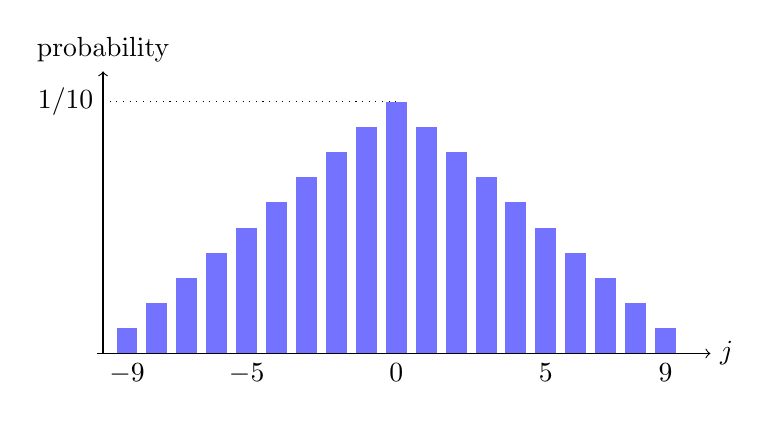
\begin{tikzpicture}[x=.38cm,y=32cm]
\draw[->] (-10,0)--(10.5,0) node[right] {$j$};
\draw[->] (-9.8,0)--(-9.8,.112) node[above] {probability};
\foreach \j in {-9,-8,...,9}{\pgfmathsetmacro{\hh}{(10-abs(\j))/100}\fill[blue!55] (\j-.35,0) rectangle (\j+.35,\hh);}
\foreach \j in {-9,-5,0,5,9}{\node[below] at (\j,0) {$\j$};}
\draw[dotted] (-9.8,.1)--(0,.1);
\node[left] at (-9.8,.1) {$1/10$};
\end{tikzpicture}
